\documentclass{beamer}
\usepackage[utf8]{inputenc}
\usepackage[T1]{fontenc}

\title{Project Report}
\subtitle{\textit{Week 2}}
\date[]{2024/2025}
\author[Fritz]{Fritz Adelbertus Sitindaon}

\usetheme{Warsaw}
\setbeamertemplate{footline}[frame number]
% ===== Setup Font =====
\usepackage[sfdefault,lf]{carlito}
\usepackage[T1]{fontenc}
\renewcommand*\oldstylenums[1]{\carlitoOsF #1}

% ==== Import Math Packages =====
\usepackage{amsmath, amssymb, amsthm}
\usepackage{mathtools}

% ==== There required =====
\usepackage[dvipsnames]{xcolor}
\usepackage[most]{tcolorbox}
\def\wallpaper{wallpaper.jpg}

\def\R{\mathbb{R}}
\def\P{\mathbb{P}}
\def\N{\mathbb{N}}
\def\O{\mathbb{O}}


\def\nX{\mathcal{X}}
\def\nY{\mathcal{Y}}
\def\nT{\mathcal{T}}
\def\nU{\mathcal{U}}
\def\nB{\mathcal{B}}
\def\nS{\mathcal{S}}
\def\nP{\mathcal{P}}
\def\nA{\mathcal{A}}
\def\nF{\mathcal{F}}
\newcommand{\comp}[1]{\overline{#1}} 

\DeclarePairedDelimiter\abs{\lvert}{\rvert}
\DeclarePairedDelimiter\floor{\lfloor}{\rfloor}
\DeclarePairedDelimiter\cic{[ }{] }
\DeclarePairedDelimiter\oic{( }{] }
\DeclarePairedDelimiter\cio{[ }{) }
\DeclarePairedDelimiter\oio{( }{) }
\DeclarePairedDelimiter\set{\{ }{\} }
\DeclarePairedDelimiter\brk{(}{)}
\DeclarePairedDelimiter\seq{\langle}{\rangle}

\begin{document}

\begin{frame}
\titlepage
\end{frame}


\begin{frame}{This Week Main Problem}
    \begin{itemize}
        \item COMCOT dapat mensimulasikan banyak scenario tsunami.
        \item Banyak if/else dan switch cases. Beberapa if/else juga nested sehingga
        meningkatkan kompleksitas program.
        \item Mempersulit memahami ide dari suatu fungsi/prosedur
    \end{itemize}
\end{frame}

\begin{frame}{Current Solution}
    \begin{itemize}
        \item Create a minimal working program. 
        \item Focus on one tsunami scenario.
        \item Expand to other scenario after the program works.
    \end{itemize}
\end{frame}


\begin{frame}{Porting $type\_module.f90$ ke typemodule.hs}
    \begin{itemize}
        \item $type\_module.f90$ berisi struktur data yang digunakan pada program
        \item data yang digunakan pada program ini menyerupai dictionary di python (hash tables)
    \end{itemize}
\end{frame}

\begin{frame}{Porting $type\_module.f90$ ke typemodule.hs}
    $LAYER$
    \begin{itemize}
        \item $LAYER$ berisi informasi dari section $layer$ pada input beserta 
        semua informasi untuk menyimpan dan mengubah grid yang merepresentasikan layer.
        \item Pada $haskell$ dibuat data type $layer$ dalam bentuk record. 
    \end{itemize}
    \begin{center}
        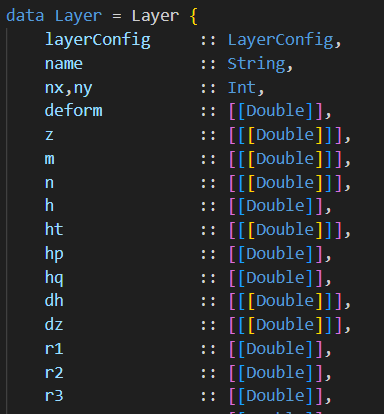
\includegraphics[scale=0.5]{figure/tmodule1.png}
    \end{center}
   
\end{frame}

\begin{frame}{Porting $type\_module.f90$ ke typemodule.hs}
    $LayerConfig$ \& $FaultConfig$
    \begin{itemize}
        \item Kedua datatype ini untuk merepresentasikan semua informasi yang diberikan
        input.
    \end{itemize}
    \begin{center}
        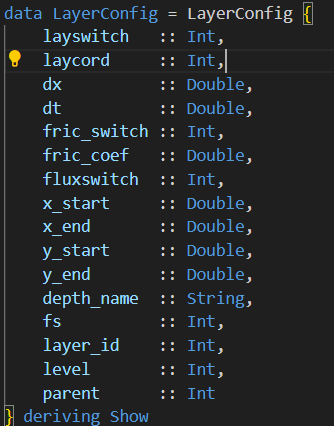
\includegraphics[scale=0.5]{figure/tmodule2.png}
        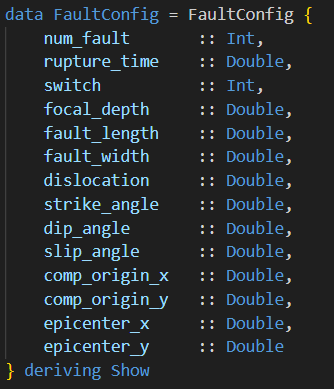
\includegraphics[scale=0.5]{figure/tmodule3.png}
    \end{center}
\end{frame}

\begin{frame}{Porting $mass.f90$ ke mass.hs}
    Tujuan pada module ini adalah menyelesaikan persamaan berikut
    \begin{center}
        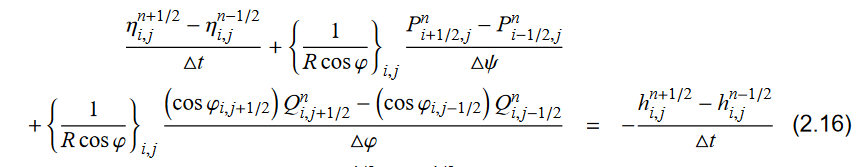
\includegraphics[scale=0.4]{figure/mass.png}
    \end{center}
    \begin{center}
        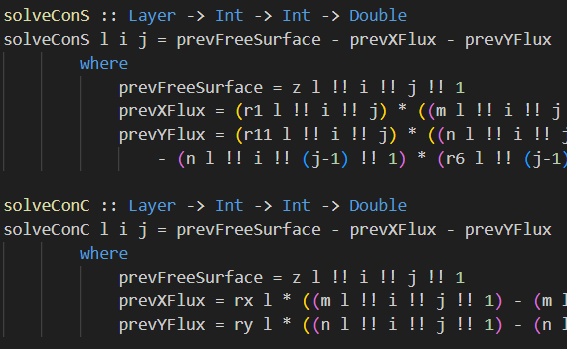
\includegraphics[scale=0.5]{figure/mass4.png}
    \end{center}
\end{frame}

\begin{frame}{Porting $mass.f90$ ke mass.hs}
    Ini diselesaikan pada setiap grid cell dalam satu time-step
    \begin{center}
        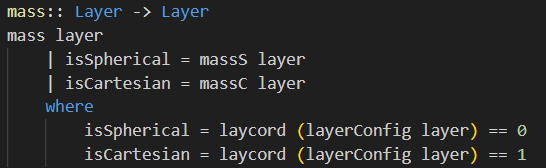
\includegraphics[scale=0.5]{figure/mass1.png}
    \end{center}
    \begin{center}
        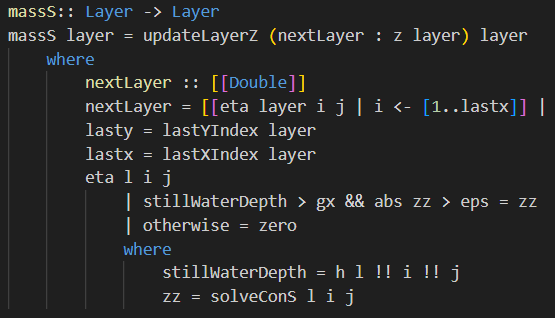
\includegraphics[scale=0.5]{figure/mass2.png}
    \end{center}
\end{frame}

\begin{frame}{Porting $moment.f90$ ke moment.hs}
    Tujuan pada module ini adalah menyelesaikan persamaan berikut
    \begin{center}
        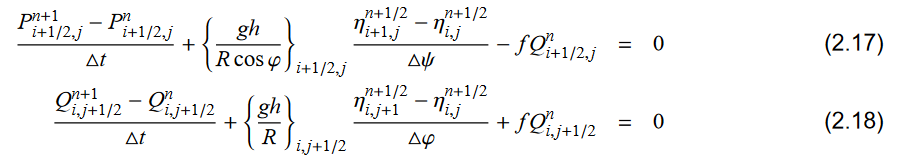
\includegraphics[scale=0.4]{figure/moment.png}
    \end{center}
    \begin{center}
        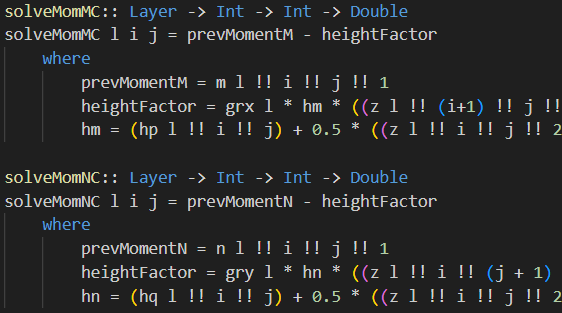
\includegraphics[scale=0.5]{figure/moment1.png}
    \end{center}
\end{frame}

\begin{frame}{Porting $moment.f90$ ke moment.hs}
    Ini diselesaikan pada setiap grid cell dalam satu time-step
    \begin{center}
        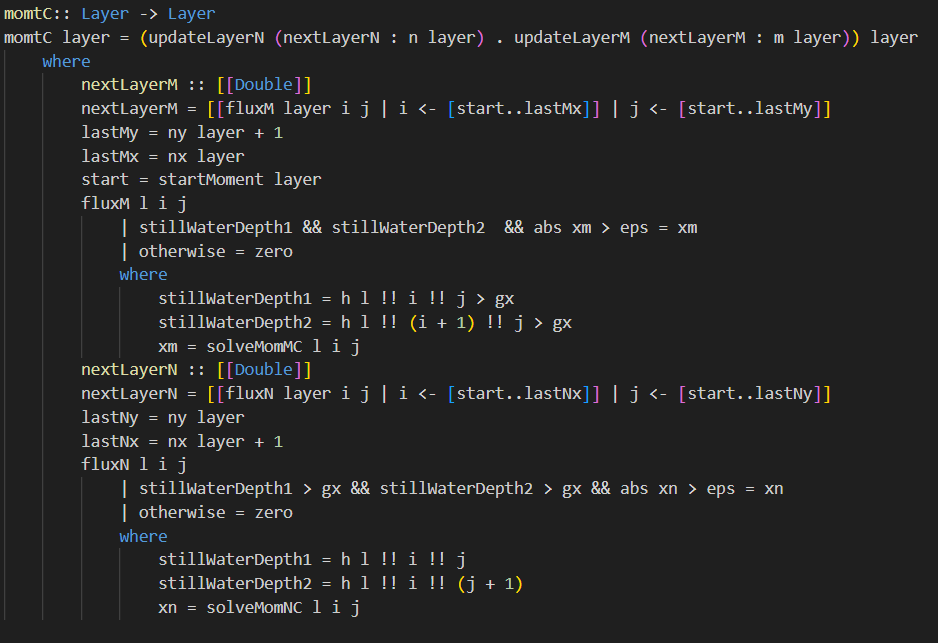
\includegraphics[scale=0.4]{figure/moment2.png}
    \end{center}
\end{frame}

\begin{frame}{Porting $deform.f90$ ke deform.hs}
    \begin{itemize}
        \item Deformasi menggunakan model Okada untuk menghasilkan gelombang awal
        \item Rumusnya tidak dijabarkan pada manual COMCOT
        \item 4 fungsi diport dari .f90 dimana 1 fungsi adalah model Okada dan
        3 lainnya adalah fungsi yang dipanggil pada model Okada
    \end{itemize}
    \begin{center}
        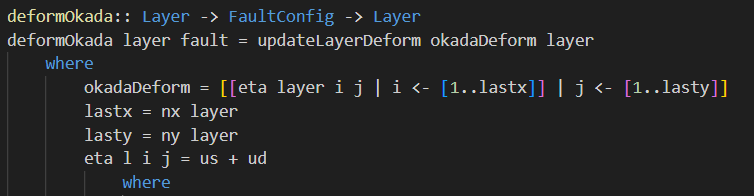
\includegraphics[scale=0.5]{figure/deform1.png}
    \end{center}
\end{frame}

\begin{frame}{Porting $deform.f90$ ke deform.hs}
    \begin{center}
        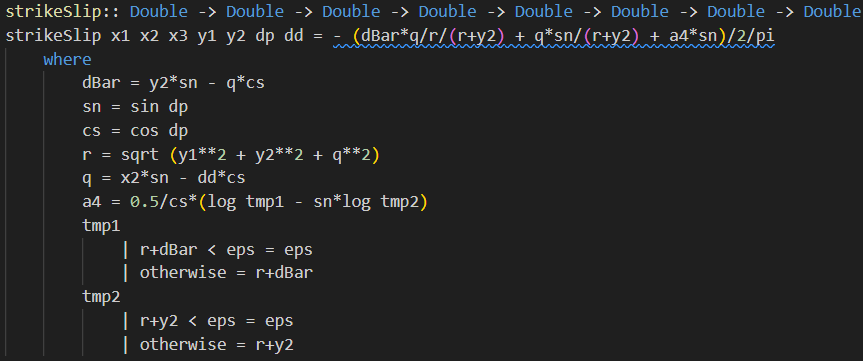
\includegraphics[scale=0.4]{figure/deform2.png}
    \end{center}
    \begin{center}
        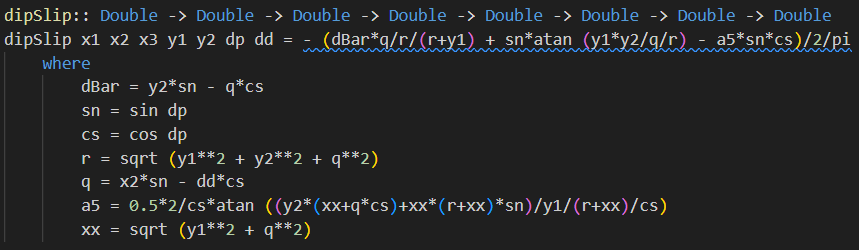
\includegraphics[scale=0.4]{figure/deform3.png}
    \end{center}
\end{frame}

\begin{frame}{Porting $deform.f90$ ke deform.hs}
    \begin{center}
        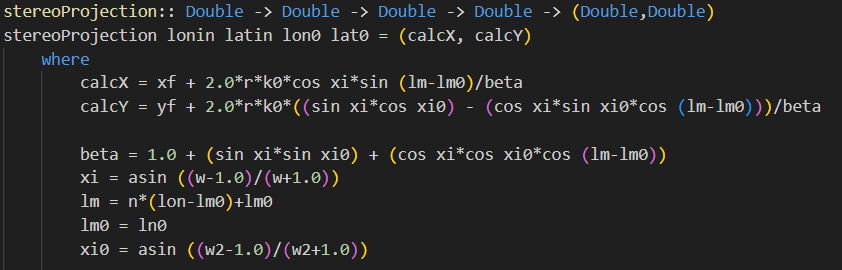
\includegraphics[scale=0.4]{figure/deform4.png}
    \end{center}
\end{frame}


\begin{frame}{File Structure and Size}
    \begin{itemize}
        \item $type\_module.f90$: 180 lines
        \item $initialization.f90$: 2021 lines
        \item $all\_grids.f90$: 927 lines
        \item $boundaries.f90$: 439 lines
        \item $comcot.f90$: 526 lines
        \item $wavemaker.f90$: 362 lines
        \item $deform.f90$: 675 lines
        \item $landslide.f90$: 299 lines
        \item $mass.f90$: 205 lines
        \item $moment.f90$: 939 lines
        \item $dispersion.f90$: 1647 lines
        \item $hotstart.f90$: 138 lines
        \item $output.f90$: 1010 lines
    \end{itemize}
\end{frame}

\begin{frame}{Progress (compared to the original source code)}
    \begin{itemize}
        \item $type\_module.f90$: \textcolor{green}{60\%}
        \item $initialization.f90$: \textcolor{orange}{20\%}
        \item $all\_grids.f90$: \textcolor{red}{0\%}
        \item $boundaries.f90$: \textcolor{red}{0\%}
        \item $comcot.f90$: \textcolor{red}{0\%}
        \item $wavemaker.f90$: \textcolor{red}{0\%}
        \item $deform.f90$: \textcolor{green}{50\%}
        \item $landslide.f90$: \textcolor{red}{0\%}
        \item $mass.f90$: \textcolor{green}{50\%}
        \item $moment.f90$: \textcolor{orange}{30\%}
        \item $dispersion.f90$: \textcolor{red}{0\%}
        \item $hotstart.f90$: \textcolor{red}{0\%}
        \item $output.f90$: \textcolor{red}{0\%}
    \end{itemize}
\end{frame}

\begin{frame}{Progress (compared to the minimal working program)}
    \begin{itemize}
        \item $type\_module.f90$: \textcolor{green}{100\%}
        \item $initialization.f90$: \textcolor{orange}{40\%}
        \item $all\_grids.f90$: \textcolor{red}{0\%}
        \item $boundaries.f90$: \textcolor{red}{0\%}
        \item $comcot.f90$: \textcolor{red}{0\%}
        \item $deform.f90$: \textcolor{green}{80\%}
        \item $mass.f90$: \textcolor{green}{100\%}
        \item $moment.f90$: \textcolor{green}{100\%}
        \item $output.f90$: \textcolor{red}{0\%}
    \end{itemize}
\end{frame}

\begin{frame}{Next Target (compared to the minimal working program)}
    \begin{itemize}
        \item $type\_module.f90$: \textcolor{green}{100\%}
        \item $initialization.f90$: \textcolor{green}{90\%}
        \item $all\_grids.f90$: \textcolor{green}{90\%}
        \item $boundaries.f90$: \textcolor{green}{90\%}
        \item $comcot.f90$: \textcolor{green}{90\%}
        \item $deform.f90$: \textcolor{green}{90\%}
        \item $mass.f90$: \textcolor{green}{100\%}
        \item $moment.f90$: \textcolor{green}{100\%}
        \item $output.f90$: \textcolor{green}{90\%}
    \end{itemize}
\end{frame}

\end{document}